\documentclass[12pt]{article}

% --- Packages ---
\usepackage[utf8]{inputenc}
\usepackage[margin=1in]{geometry}
\usepackage{amsmath, amssymb}
\usepackage{array} 
\usepackage{booktabs}
\usepackage{enumitem}
\usepackage{fancyhdr}
\usepackage{float}
\usepackage{graphicx}
\usepackage{hyperref}
\usepackage{listings}
\usepackage{xcolor}

% --- References ---
% https://www.overleaf.com/learn/latex/Bibliography_management_with_biblatex
\usepackage{biblatex}
\addbibresource{references.bib}

% --- Formatting Setup ---
\hypersetup{
    colorlinks=true,
    linkcolor=blue,
    filecolor=magenta,      
    urlcolor=blue,
}

\title{CSE 554: Assignment 3}
\author{Jack Lowry, Nam Pho, Brett Saiki}
\date{March 2, 2026}

\begin{document}

\pagestyle{fancy}

\fancyhead{} % clear all header fields
\fancyhead[LO]{CSE 554: Group 14}
\fancyhead[CO]{HW3 (Winter 2026)}
\fancyhead[RO]{March 2, 2026}

\fancyfoot{} % clear all footer fields
\fancyfoot[CO]{\thepage}

\maketitle

% --- Section 1: General Matrix Multiplication ---
\section{General Matrix Multiplication}

\begin{enumerate}[label=\textbf{Q\arabic*.}]
    \item 
    \begin{enumerate}
        \item What is the operational intensity of a GEMM in terms of $M$, $N$, $K$ dimensions? \\

        Consider the GEMM operation $AB=C$ for matrices $A$, $B$, and $C$. The matrices are of sizes $(M\times K)$, $(K\times N)$, and $(M\times N)$. Each element $c_{ij}$ of matrix $C$ is a dot product
        requiring $K$ multiplications and $K - 1$ additions. This is replicated for all $MN$ elements.
        \begin{align*}
            W_{FLOPs} &= MN\left(2K-1\right)
        \end{align*}
        For the same GEMM set up to read $A$ and $B$ then write $C$ from memory requires moving the number of elements in each as the product of their dimensions. This value needs to be scaled by the byte multiple of the data type size $(S)$. For example, $S=2$ for FP16 representation of all elements and assuming all elements are of the same data type.
        \begin{align*}
            Q_{Bytes} &= S\left(MK + KN + MN\right)
        \end{align*}
        The operational intensity $(I)$ is defined as the ratio of work $(W)$ in FLOPs to the memory traffic $(Q)$ as measured in Bytes.
        \begin{align*}
            I &= \frac{W}{Q} = \boxed{\frac{MN\left(2K-1\right)}{S\left(MK + KN + MN\right)}} \text{ FLOPs per Byte}
        \end{align*}

        \item Calculate the compute intensity for $M$ in 128 to 2048 with step 128 and $(N, K) = (512, 512), (4096, 4096), (14336, 4096), (4096, 1024), (1024, 4096)$ and show the result in a table. \\

        See Table \ref{tab:gemm_intensity} below.
        \begin{table}[H]
            \centering
            \caption{Operational Intensity ($I$) for various GEMM dimensions.}
            \label{tab:gemm_intensity}
            %\small
            \begin{tabular}{r | r| r| r| r| r}
            %\hline
             & \multicolumn{5}{c}{$(N, K)$ Pairs} \\
            \hline
            %\cmidrule(lr){2-6}
            \textbf{M} & (512, 512) & (4096, 4096) & (14336, 4096) & (4096, 1024) & (1024, 4096) \\
            \hline
128 & 170.50 & 240.91 & 246.08 & 221.30 & 221.38 \\
256 & 255.75 & 455.06 & 473.86 & 389.90 & 390.05 \\
384 & 306.90 & 646.66 & 685.30 & 522.64 & 522.83 \\
512 & 341.00 & 819.10 & 882.11 & 629.85 & 630.08 \\
640 & 365.36 & 975.12 & 1065.74 & 718.25 & 718.51 \\
768 & 383.62 & 1116.95 & 1237.49 & 792.39 & 792.68 \\
896 & 397.83 & 1246.46 & 1398.46 & 855.46 & 855.78 \\
1024 & 409.20 & 1365.17 & 1549.65 & 909.78 & 910.11 \\
1152 & 418.50 & 1474.38 & 1691.91 & 957.04 & 957.39 \\
1280 & 426.25 & 1575.19 & 1826.02 & 998.54 & 998.90 \\
1408 & 432.81 & 1668.54 & 1952.65 & 1035.26 & 1035.64 \\
1536 & 438.43 & 1755.21 & 2072.42 & 1068.00 & 1068.39 \\
1664 & 443.30 & 1835.91 & 2185.87 & 1097.36 & 1097.76 \\
1792 & 447.56 & 1911.23 & 2293.48 & 1123.84 & 1124.25 \\
1920 & 451.32 & 1981.69 & 2395.70 & 1147.85 & 1148.27 \\
2048 & 454.67 & 2047.75 & 2492.91 & 1169.71 & 1170.14
            %\bottomrule
            %\hline
            \end{tabular}
        \end{table}

        \item What is \href{https://github.com/NVIDIA/cutlass}{CUTLASS}? What is \href{https://docs.nvidia.com/cuda/cublas/}{cuBLAS}? What is the key difference between them? \\

        CUTLASS and cuBLAS are both libraries for high-performance GEMM and deep learning operations. CUTLASS is an open-source C++ template library built on top of CUDA emphasizing customization. It provides specialized building blocks to can be assembled together into efficient kernels with expert knowledge. On the other hand, cuBLAS is a proprietary, pre-compiled library that is intended for off-the-shelf use.

        % cuBLAS is an NVIDIA hardware architecture optimized API for matrix operations. CUTLASS is one step lower, relative to cuBLAS, in that it provides templates for more advanced customizations and allows developers to build a cuBLAS-like functionality from primitives. cuBLAS is closed source, relying on opaque API calls and responses whereas CUTLASS is open-source to allow for deeper customization among developers. \\

    \end{enumerate}

    \item 
    \begin{enumerate}
        \item Profile the cuBLAS \texttt{cublasGEMMEx} performance for the above shapes and plot the performance. Plot one figure for one shape with the M dimension on the x-axis and TFLOPs (total compute/time) on the y-axis. Please use the profiling methods in \texttt{Section1/prof\_example.cu}. We do warmups and L2 cache flush to increase the profiling accuracy. The example plotting script is given at \texttt{Section1/plot\_gemm.py}. \\
        
        See next section below for all five combined plots. \\
        
        
        \item Profile the CUTLASS GEMM performance using the CUTLASS profiler for the above shapes. The CUTLASS profiler will iterate through all kernel implementations with different tile sizes and configurations. Use \texttt{--profiling-iterations} of 100. Profile different \texttt{--split\_k\_slices=1,2,4,8} with \texttt{--split\_k\_mode=serial}. Split $K$ will control the number of splits in $K$ dimension. For example, for GEMM shape $(128, 1024, 4096)$, when split $K$ is 4, the kernel will first treat it as 4 GEMM problems of size $(128, 1024, 1024)$ and perform a reduction to add the partial results. Take the best performance across all implementations for each GEMM shape. Plot the CUTLASS performance in the same figure as cuBLAS. \\

        
        Below are five plots for cuBLAS vs CUTLASS GEMM tests for $M$ and $K$ combinations $(N, K) = (512, 512), (4096, 4096), (14336, 4096), (4096, 1024), (1024, 4096)$ and varying $M$ in 128 to 2048 with step 128. These are Figures \ref{fig:gemm1}, \ref{fig:gemm2}, \ref{fig:gemm3}, \ref{fig:gemm4}, and \ref{fig:gemm5} below, respectively.
        
        \begin{figure}[H]
        \centering
        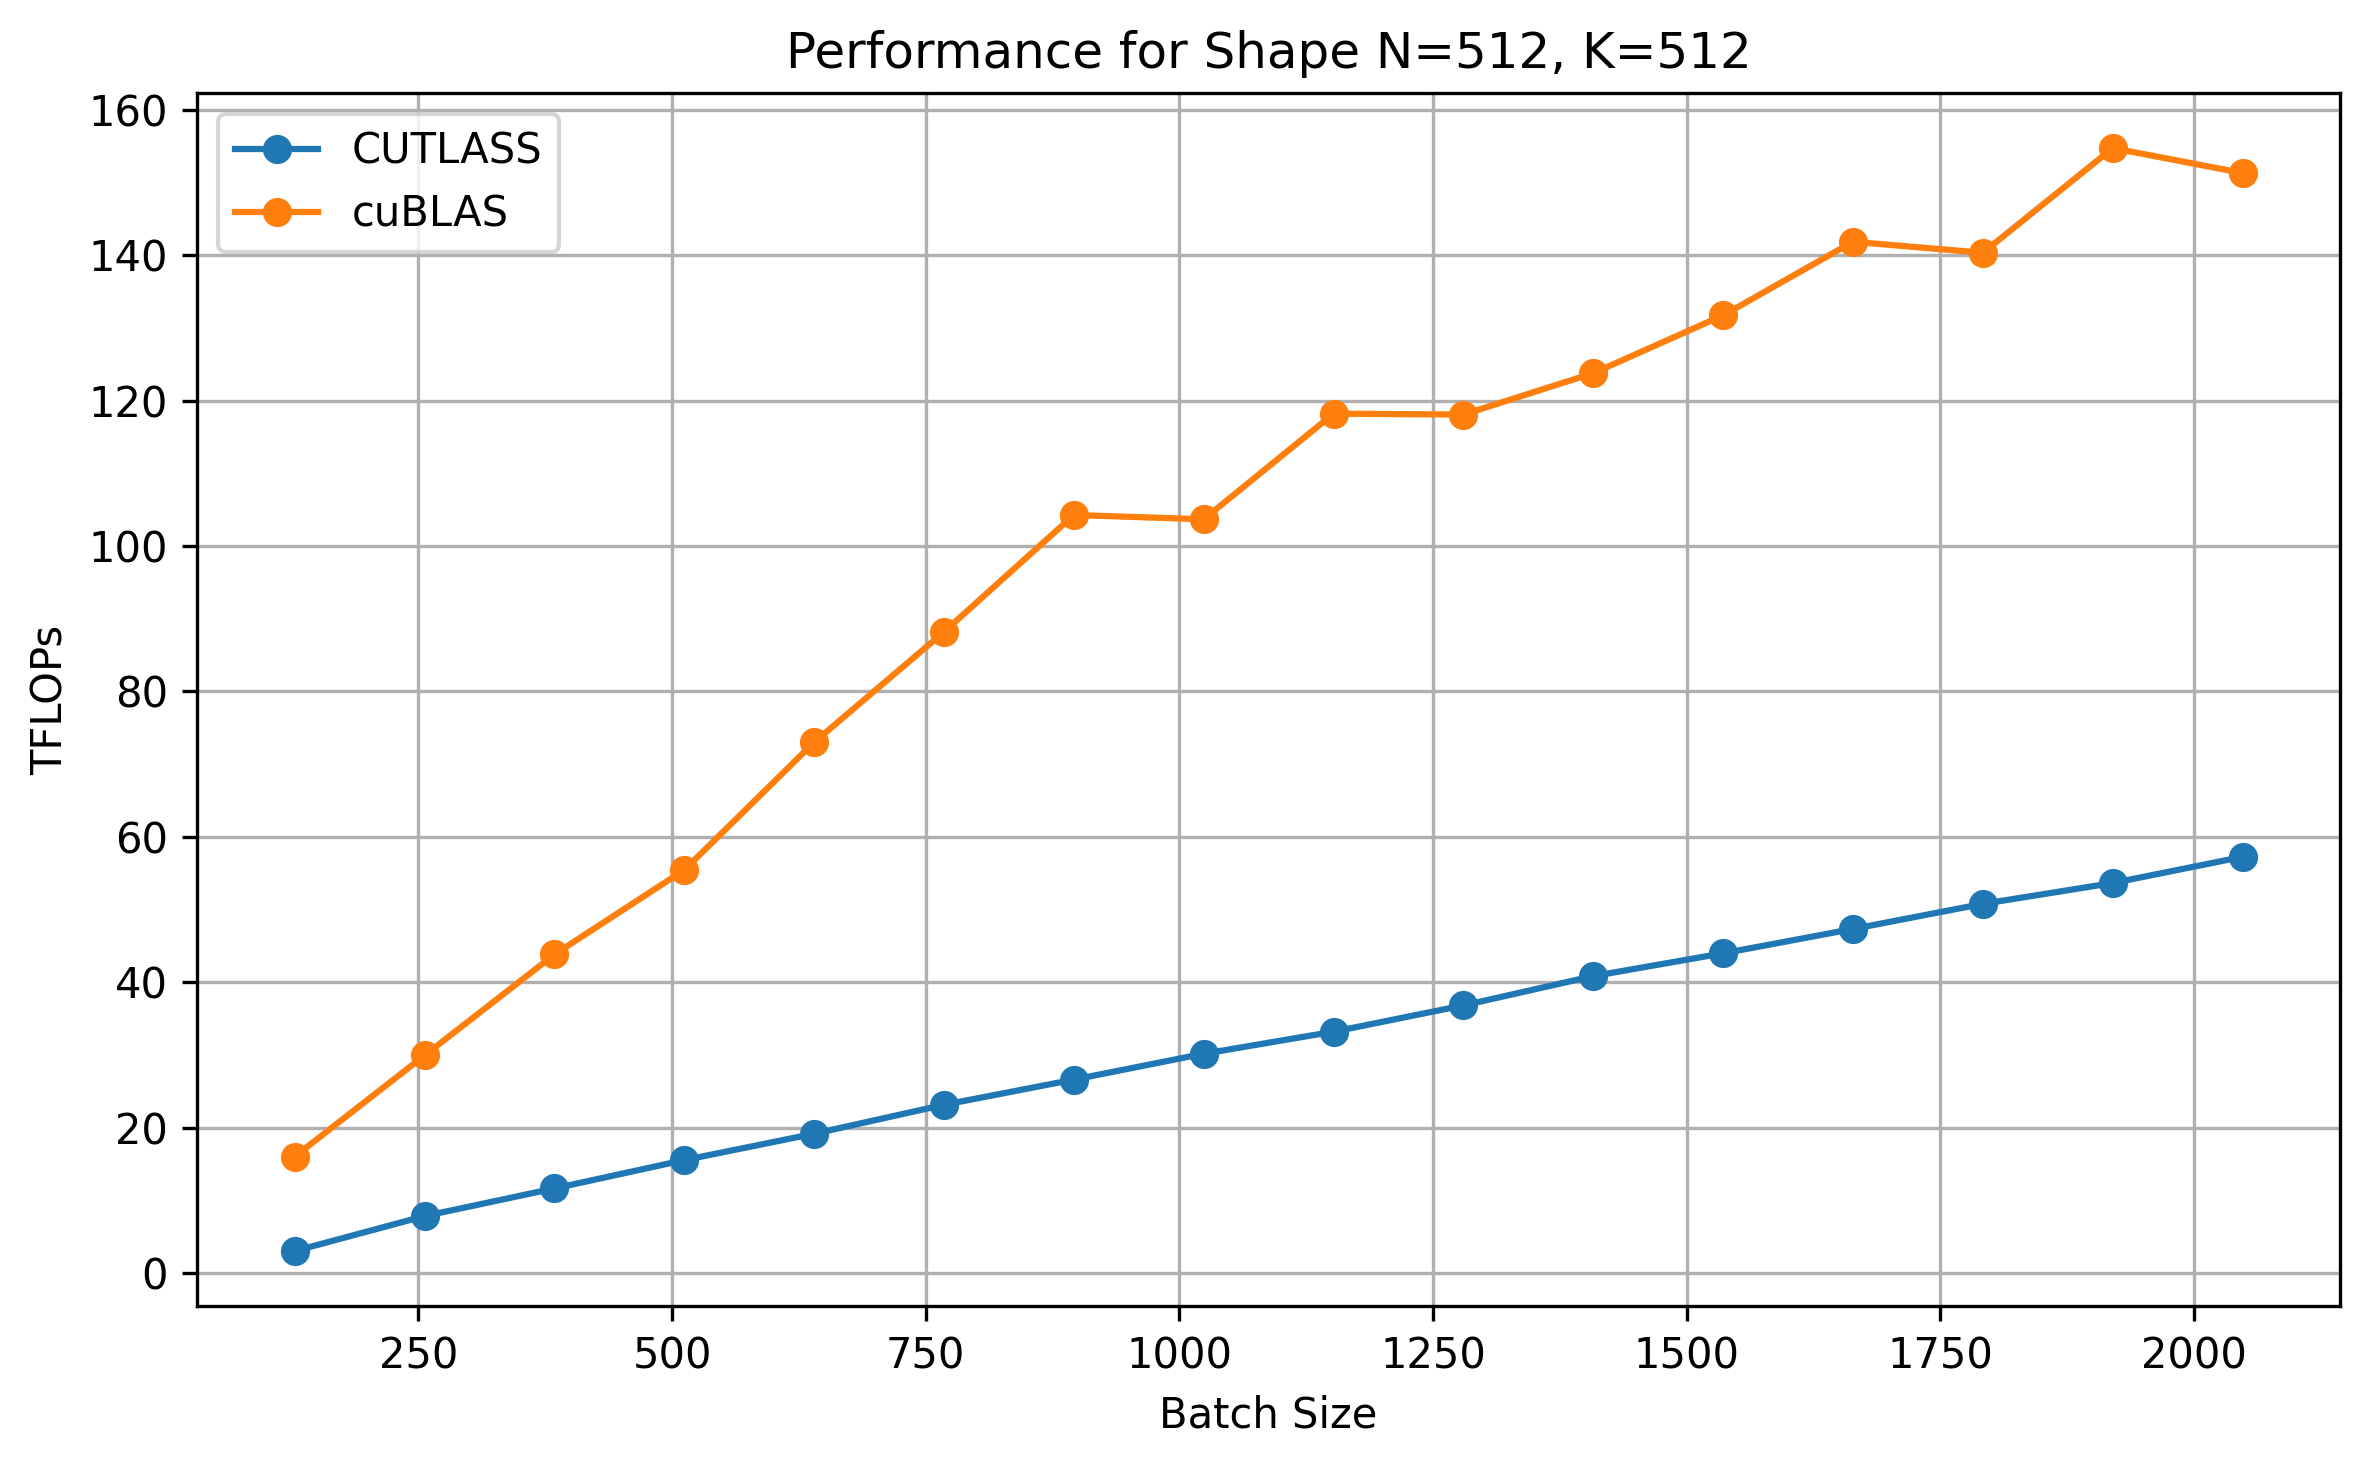
\includegraphics[width=0.9\linewidth]{fig/hw3-s1-q2-2.png}
        \caption{cuBLAS vs CUTLASS for a various batch size and $N=512$ and $K=512$.}
        \label{fig:gemm1}
        \end{figure}

        \begin{figure}[H]
        \centering
        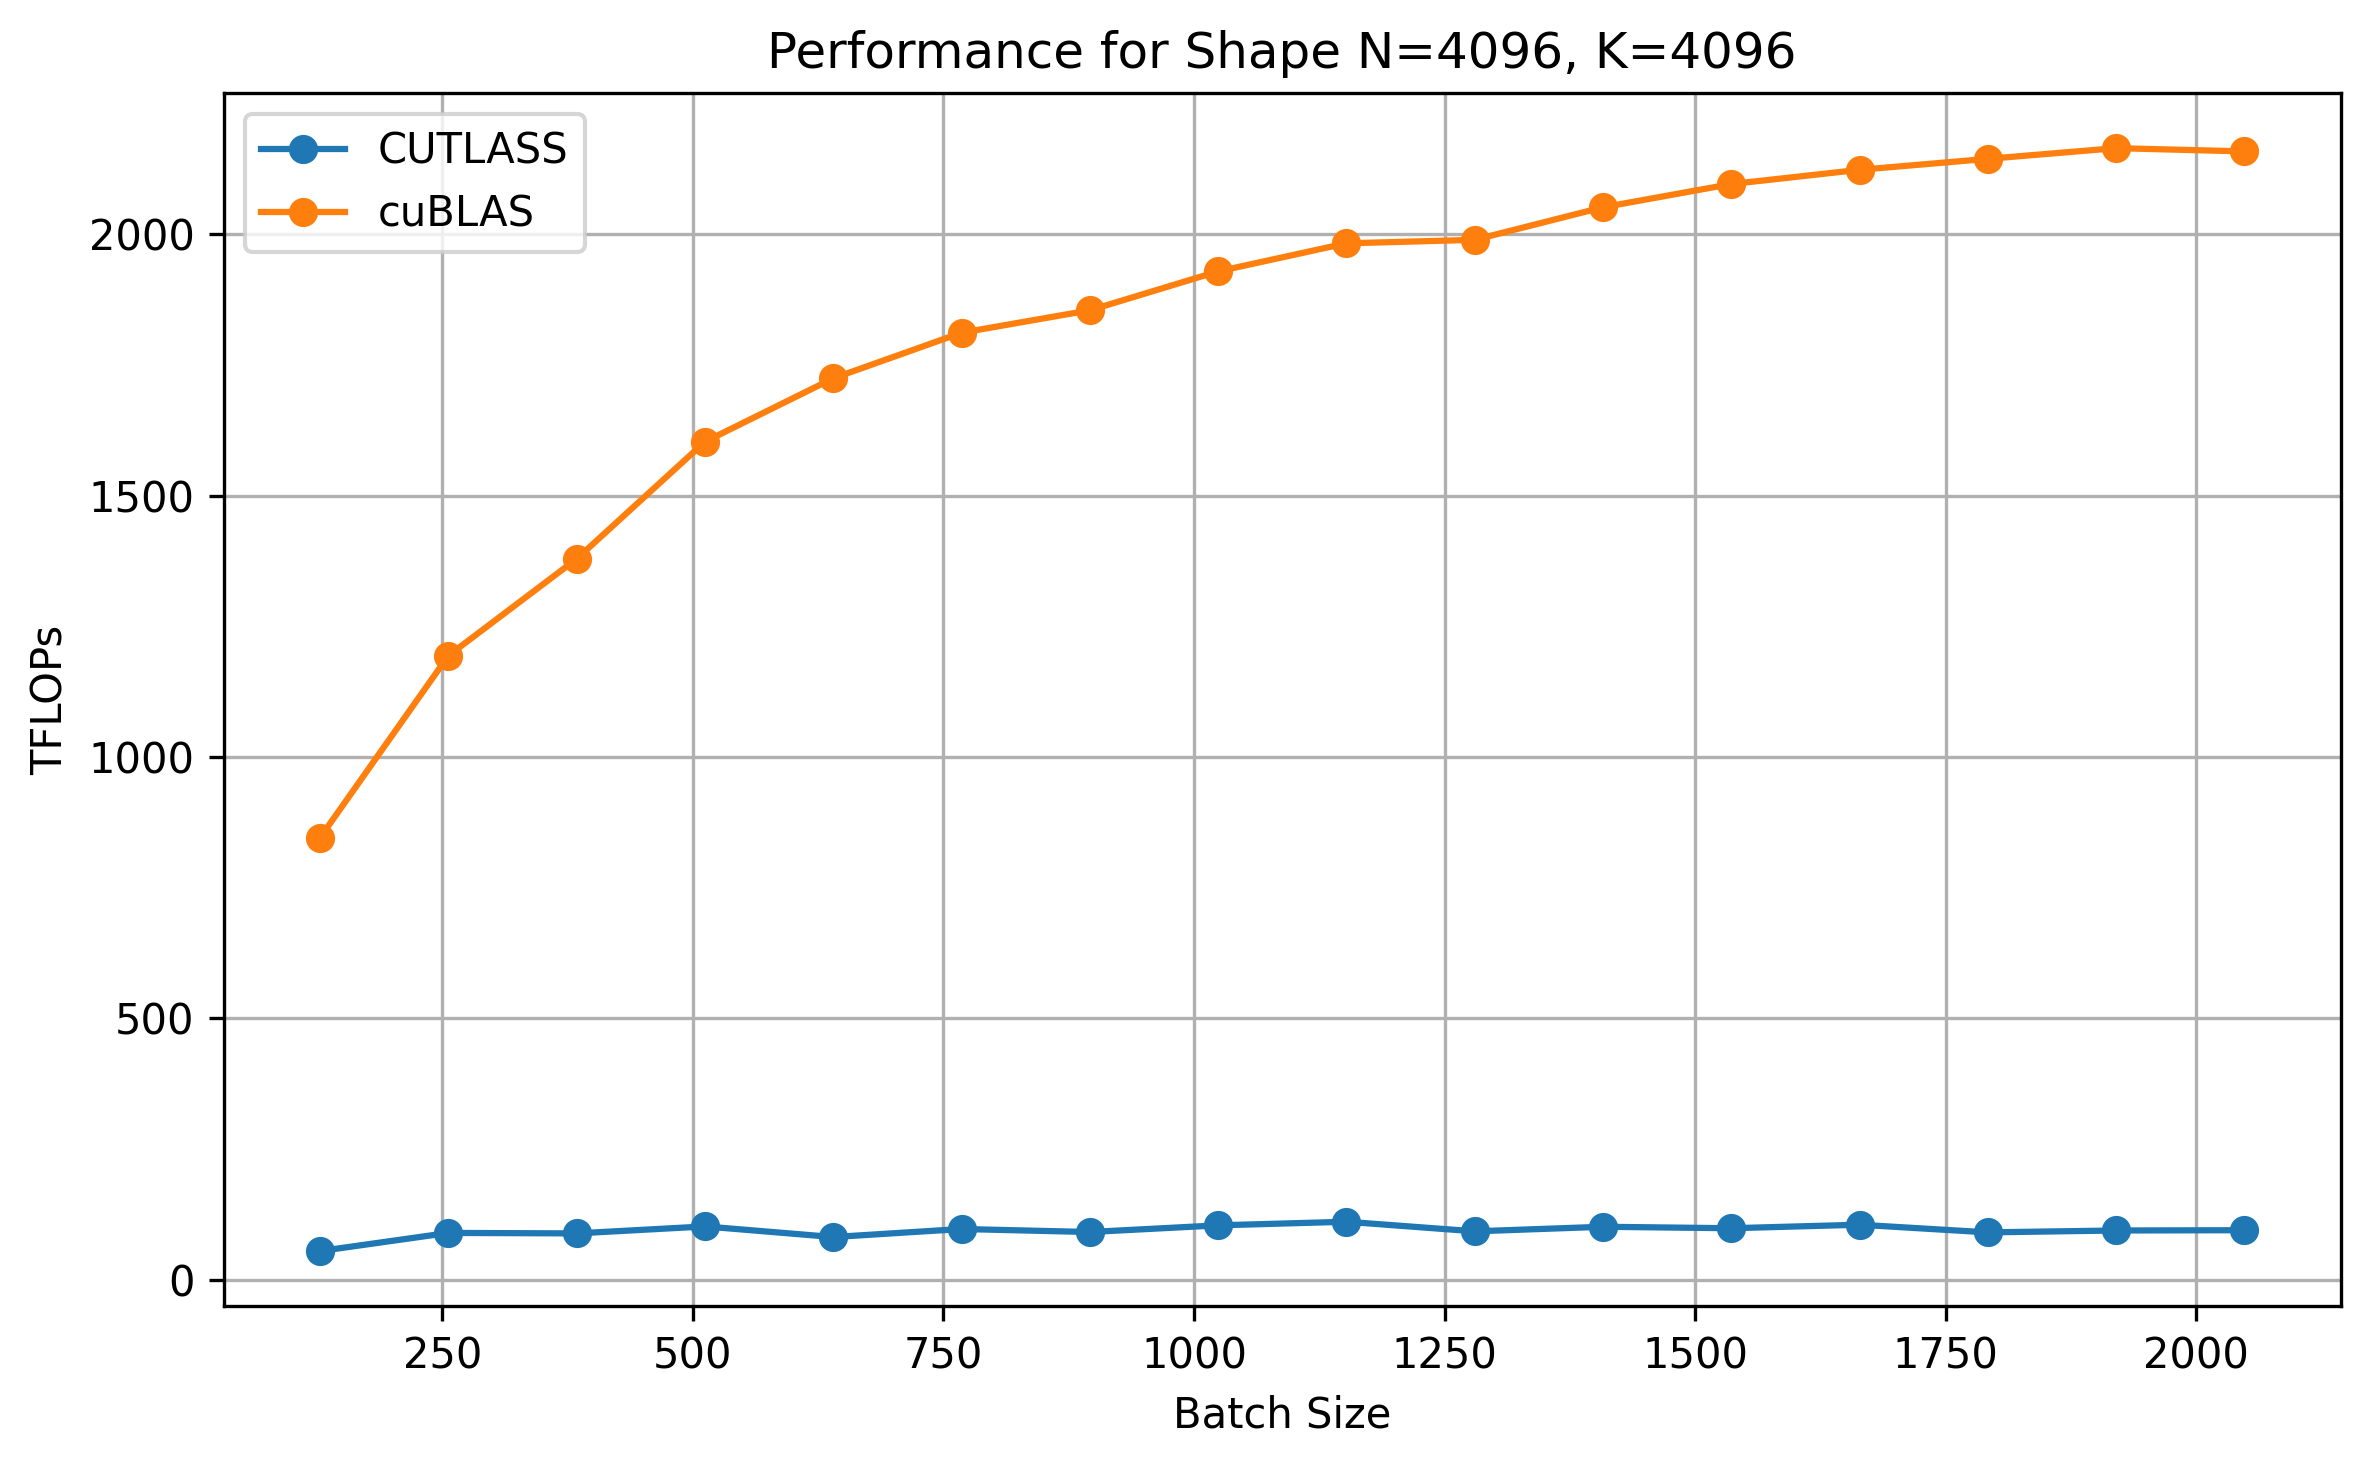
\includegraphics[width=0.9\linewidth]{fig/hw3-s1-q2-3.png}
        \caption{cuBLAS vs CUTLASS for a various batch size and $N=4096$ and $K=4096$.}
        \label{fig:gemm2}
        \end{figure}

        \begin{figure}[H]
        \centering
        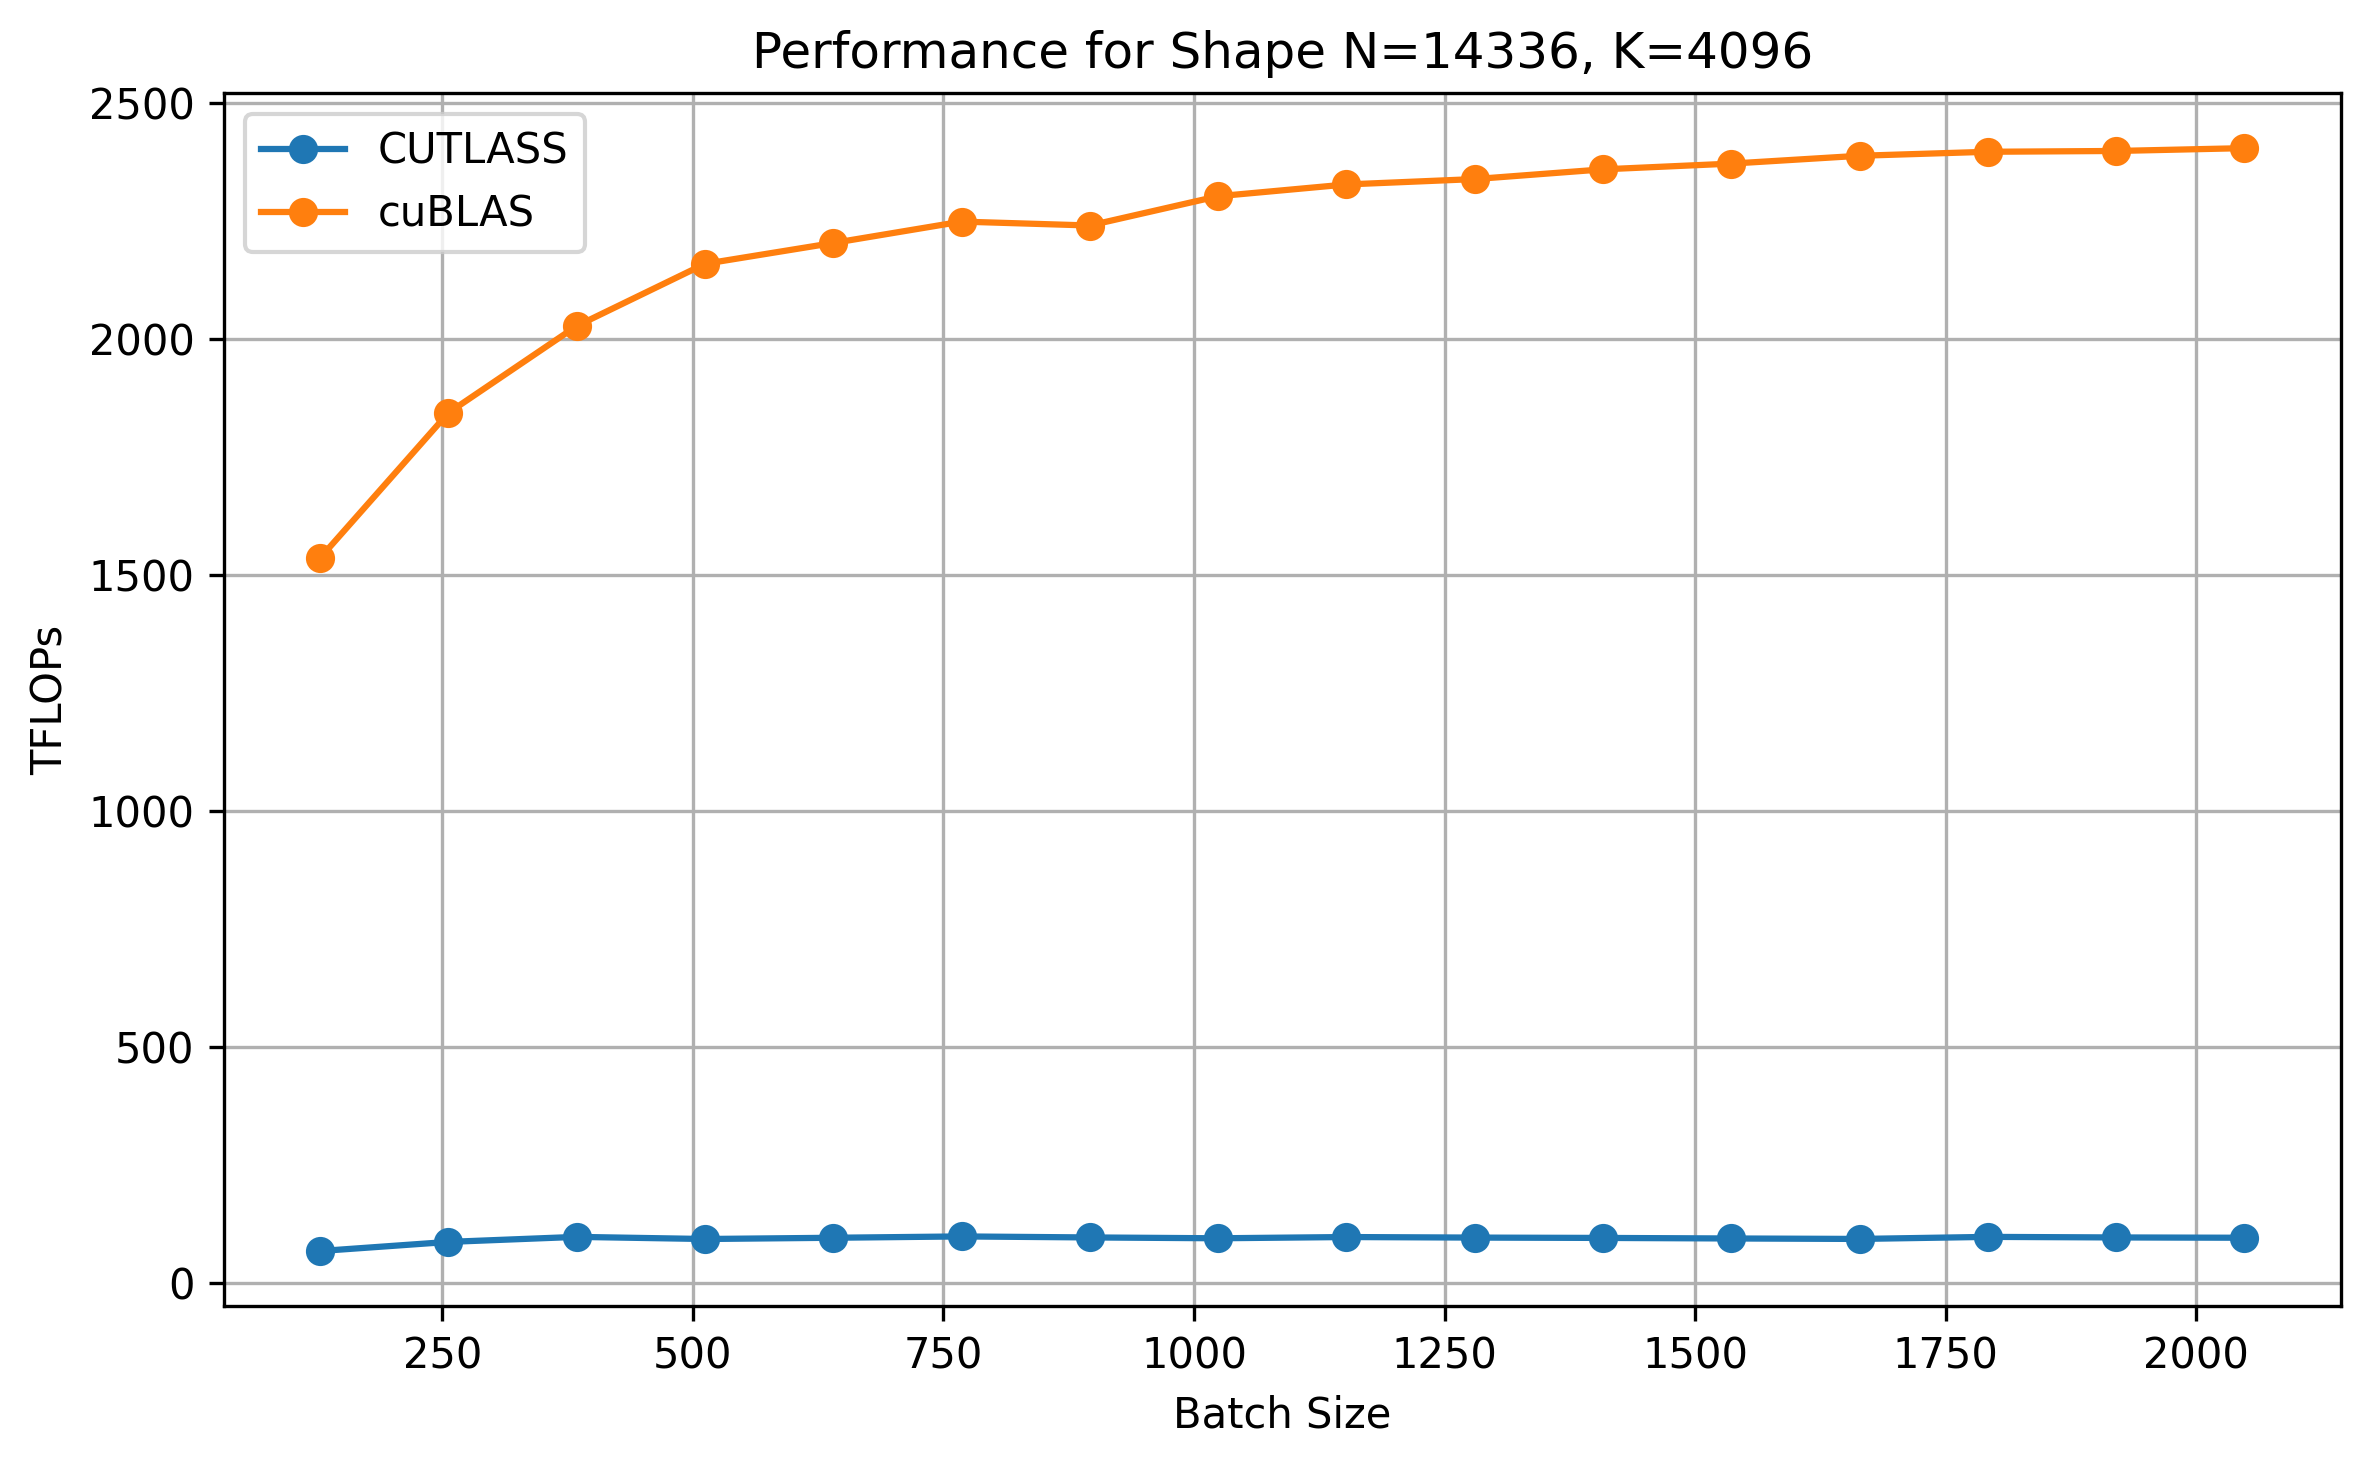
\includegraphics[width=0.9\linewidth]{fig/hw3-s1-q2-4.png}
        \caption{cuBLAS vs CUTLASS for a various batch size and $N=14336$ and $K=4096$.}
        \label{fig:gemm3}
        \end{figure}

        \begin{figure}[H]
        \centering
        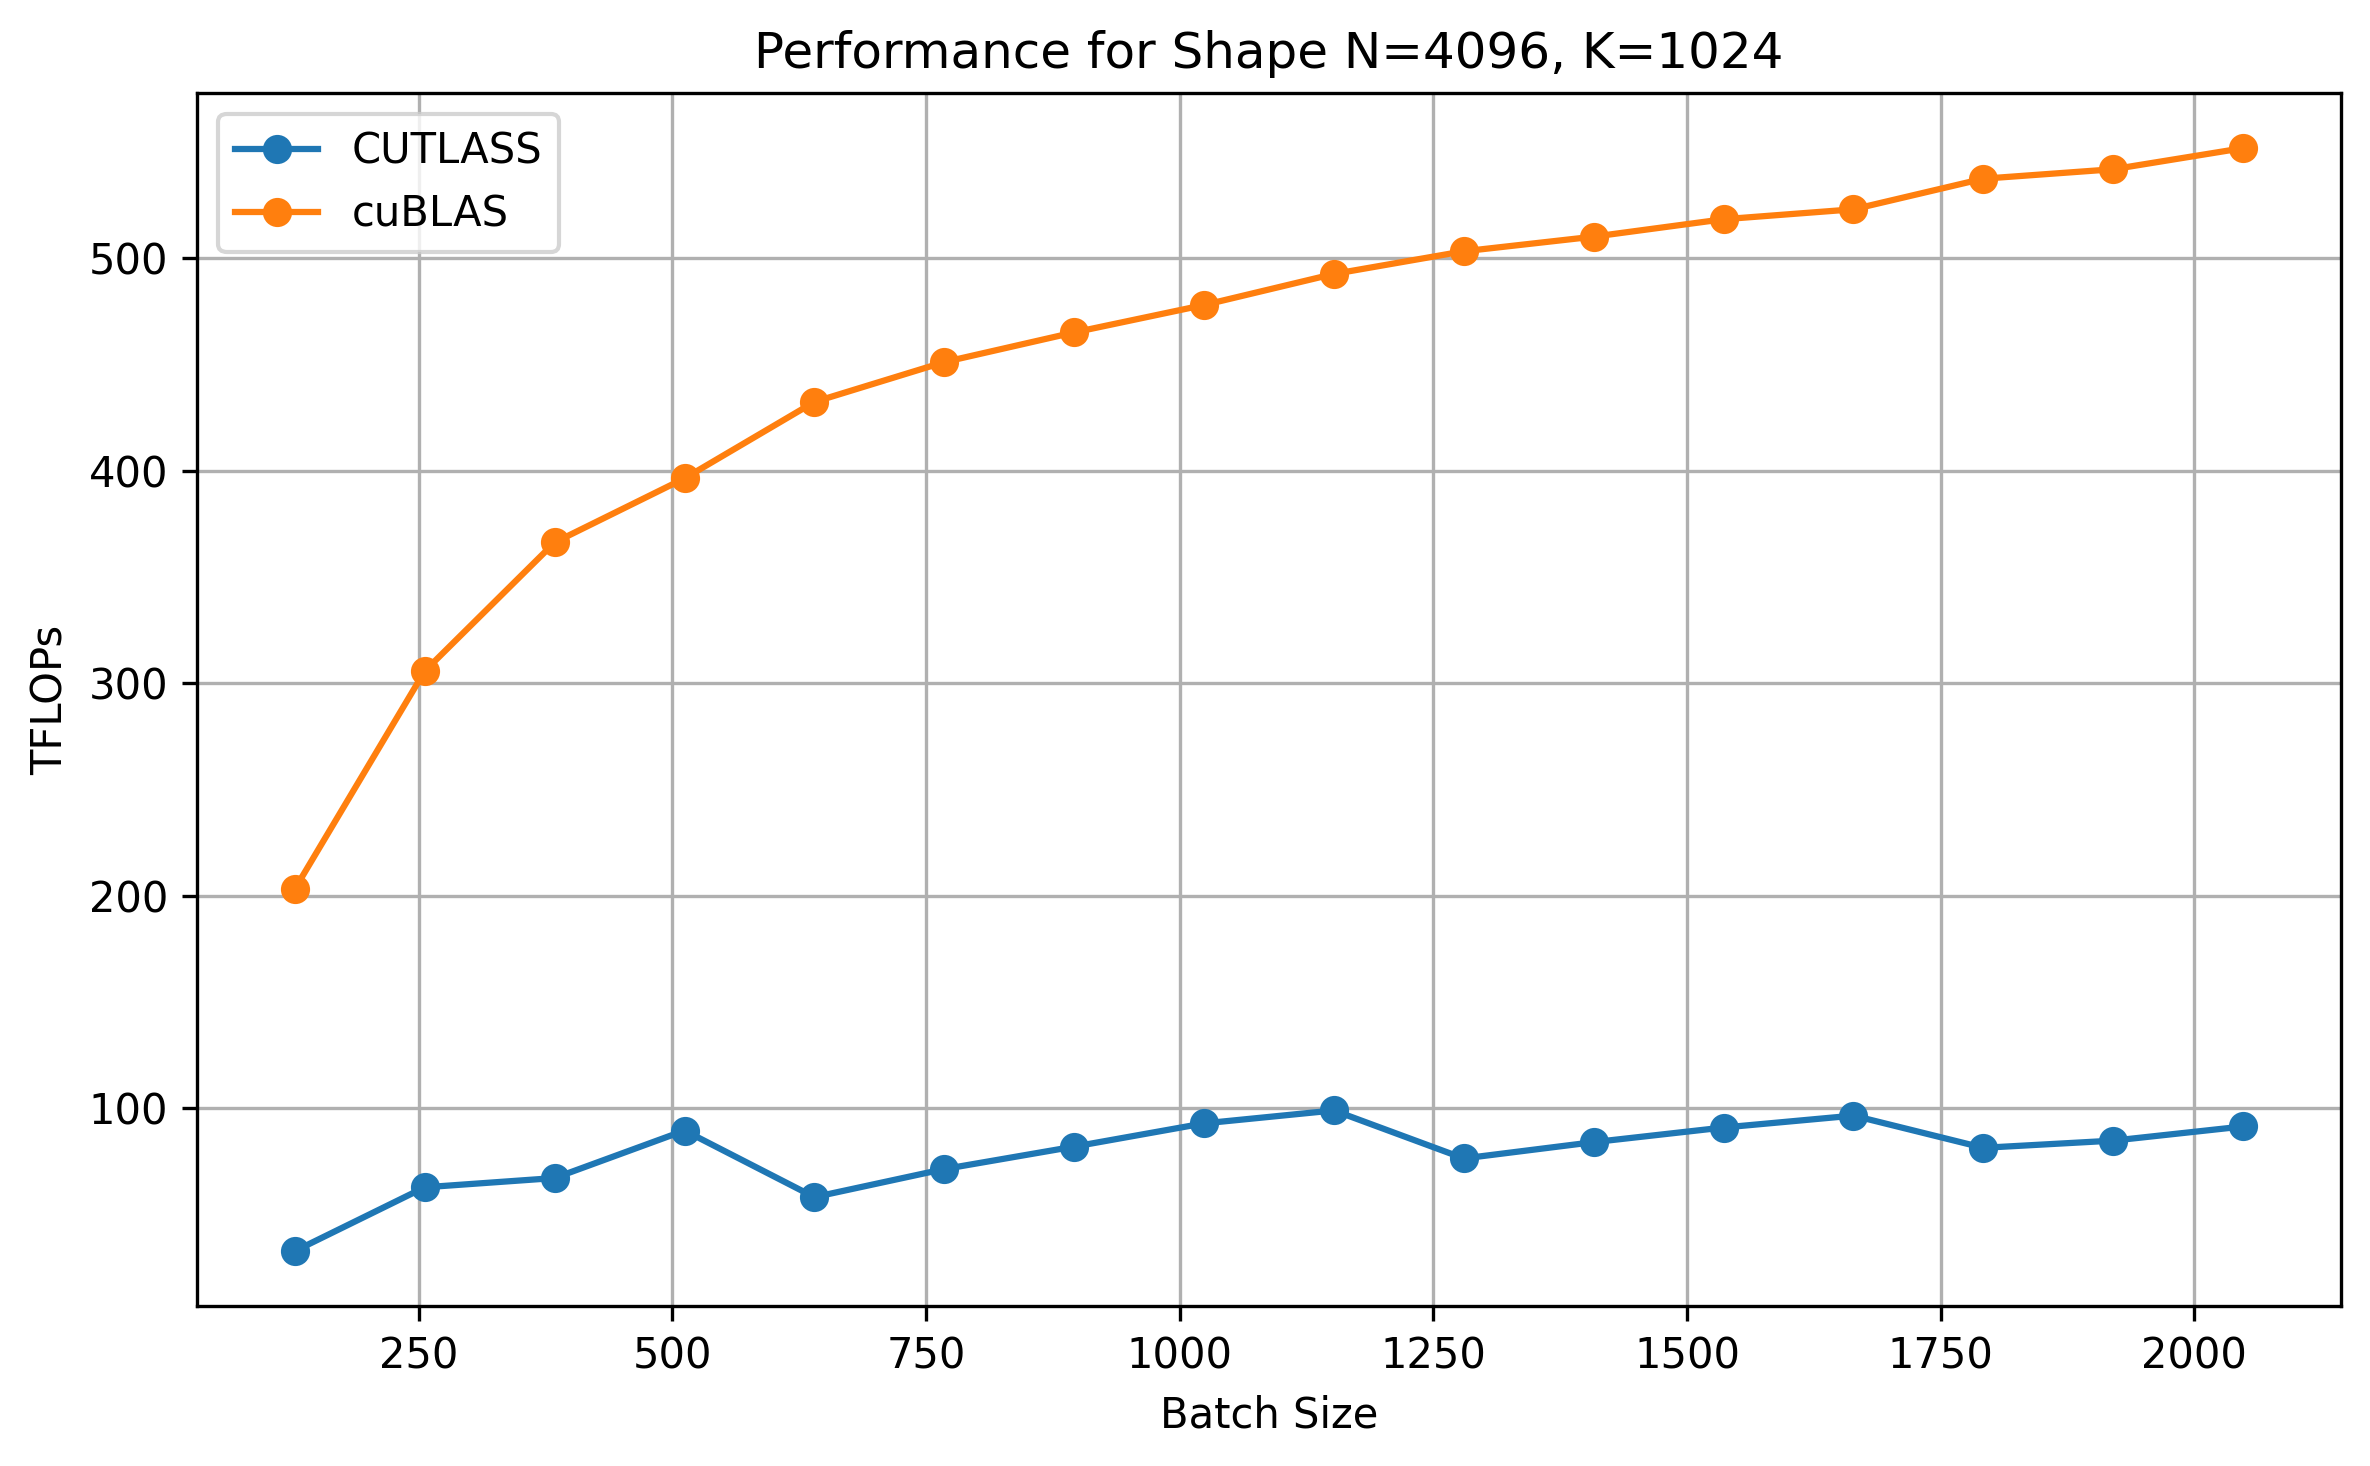
\includegraphics[width=0.9\linewidth]{fig/hw3-s1-q2-5.png}
        \caption{cuBLAS vs CUTLASS for a various batch size and $N=4096$ and $K=1024$.}
        \label{fig:gemm4}
        \end{figure}
        
        \begin{figure}[H]
        \centering
        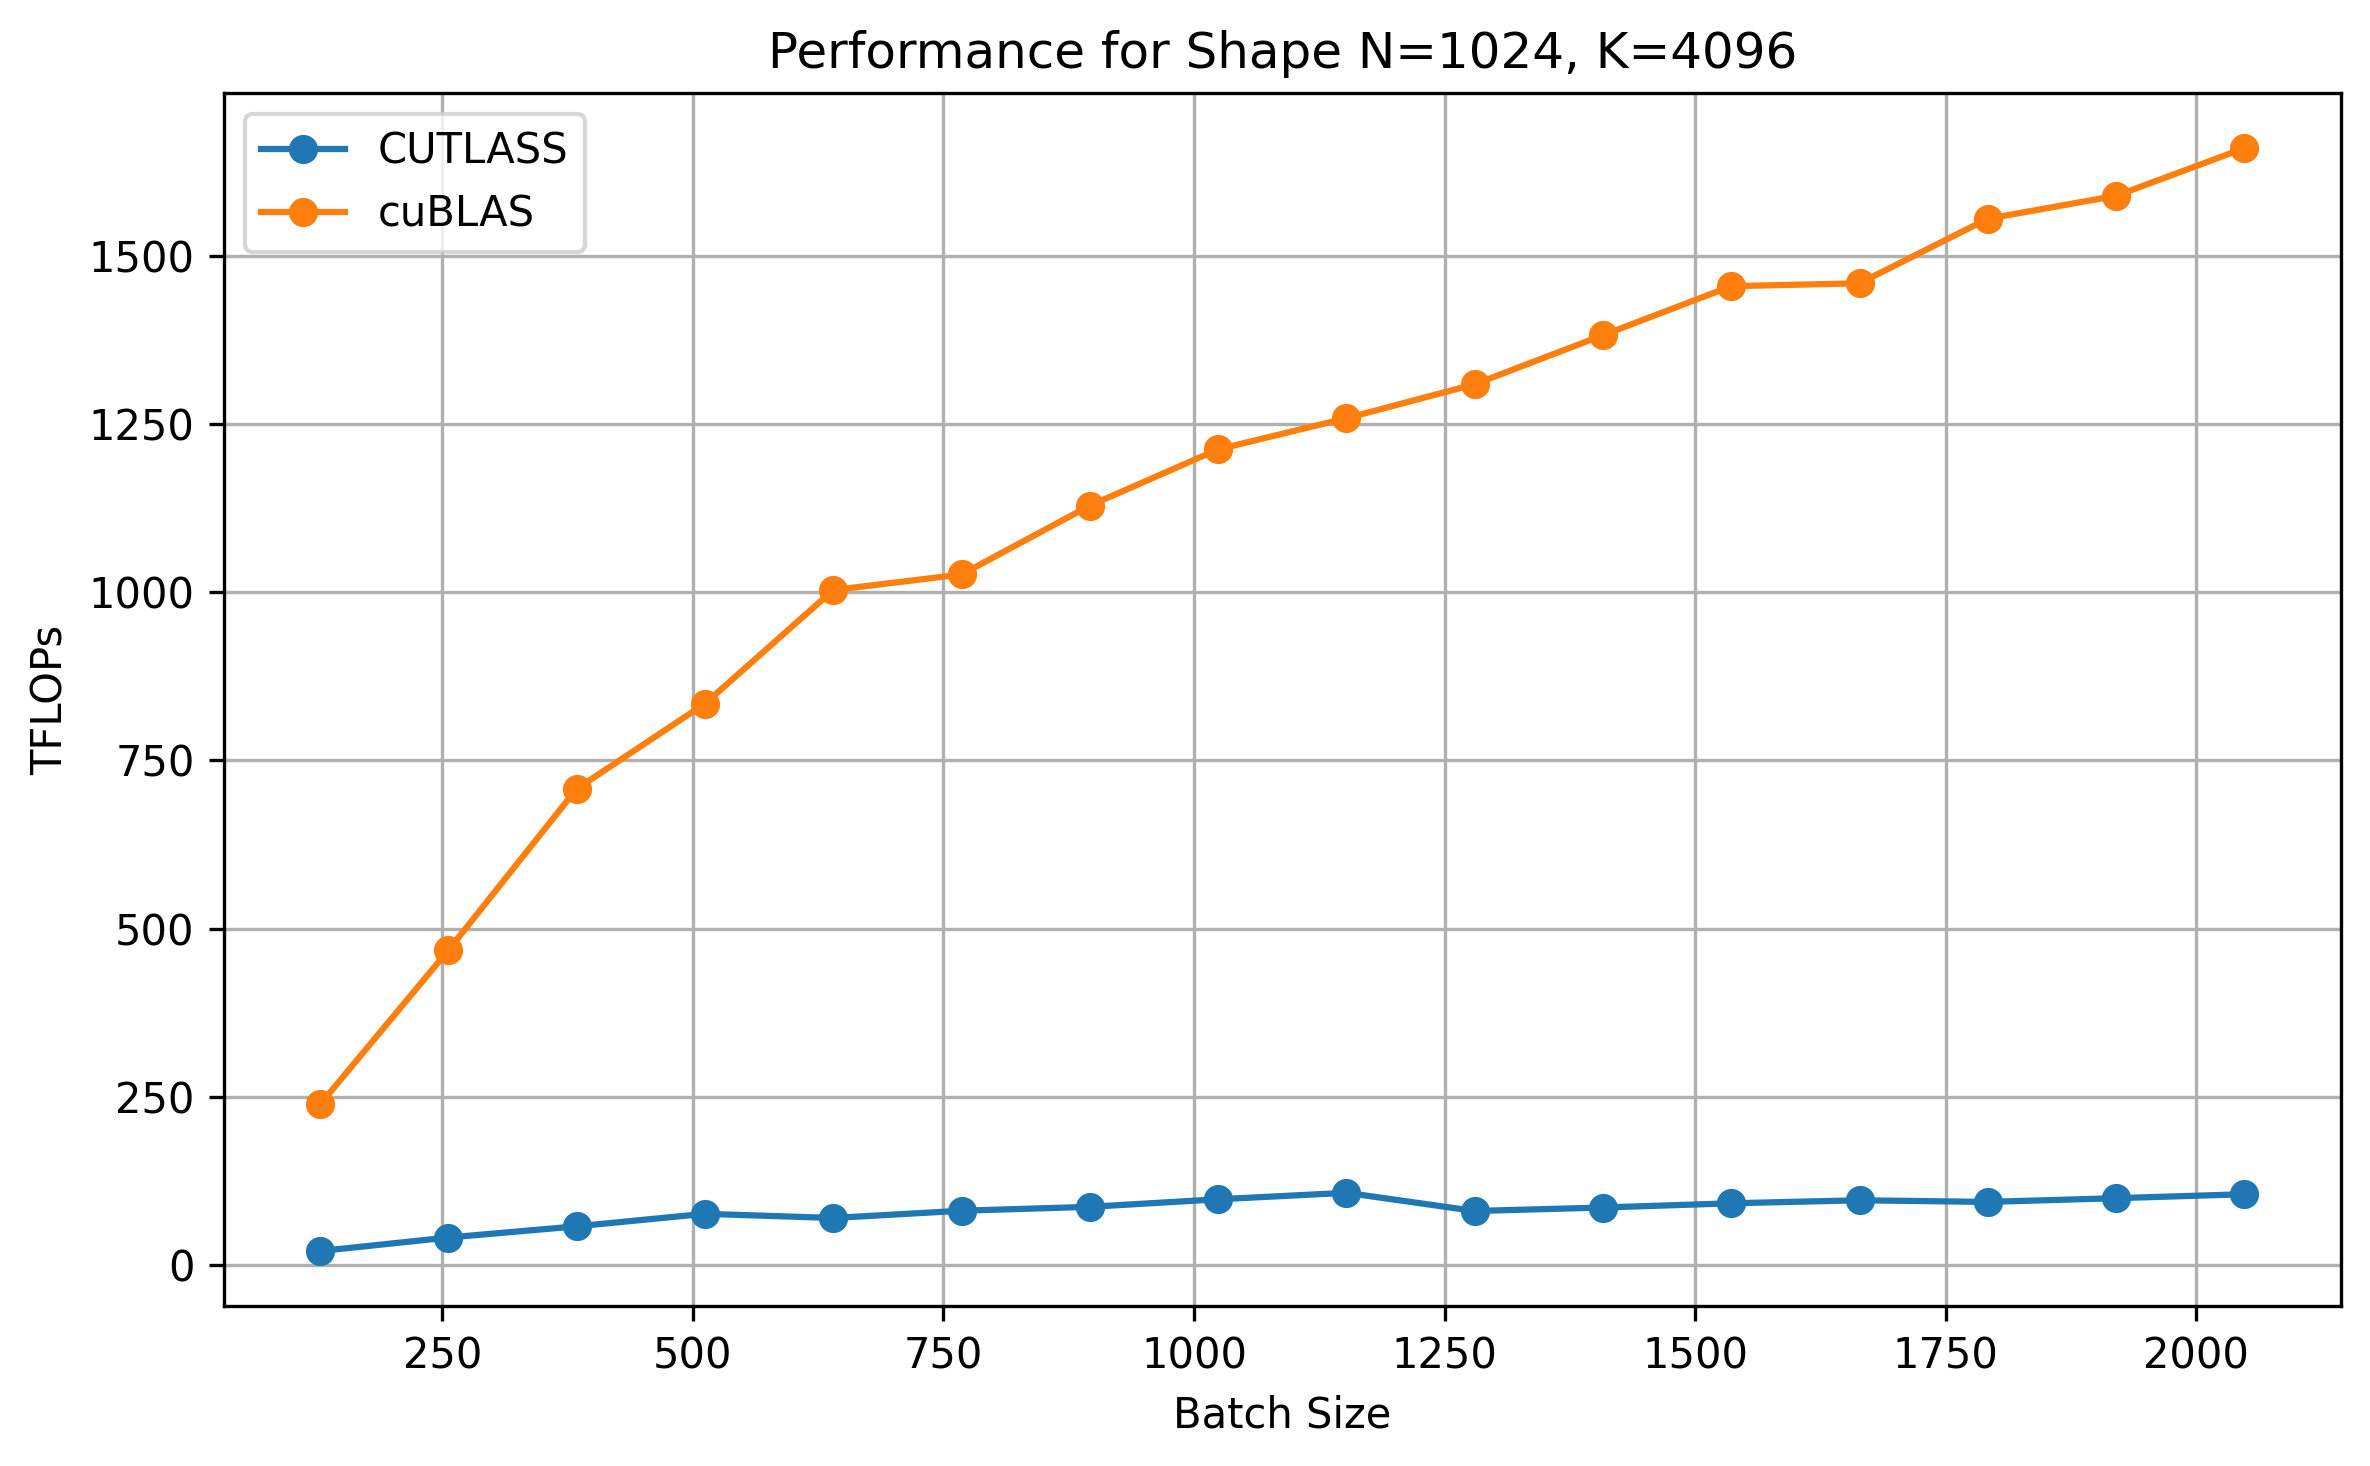
\includegraphics[width=0.9\linewidth]{fig/hw3-s1-q2-1.png}
        \caption{cuBLAS vs CUTLASS for a various batch size and $N=1024$ and $K=4096$.}
        \label{fig:gemm5}
        \end{figure}
        
        \item Investigate the kernel that achieves the best performance in CUTLASS. What is the relationship between problem size, tile size, and split $K$? \\
                    
        Maximum CUTLASS performance was achieved at 114.605 TFLOPs. The kernel was \texttt{cutlass\_tensorop\_h1688gemm\_256x128\_32x2\_nn\_align8}. The matrice dimensions were $M=1152$, $N=4096$, and $K=4096$. \\

        \item What is the difference between the CUTLASS performance and the cuBLAS performance for different shapes? Describe your findings in a few sentences. \\

        % If cuBLAS is better!
        cuBLAS outperforms CUTLASS for GEMM operations. However, for smaller sized matrices the performance gap is relatively smaller than for bigger matrices. Put another way, CUTLASS and cuBLAS can perform similarly for small matrices but performance will begin to substantially diverge with cuBLAS outperforming CUTLASS more and more as the problem size increases. \\

        % If CUTLASS is better!
        %CUTLASS almost universally outperforms cuBLAS for GEMM operations. However, for smaller sized matrices the performance gap is relatively larger than for bigger matrices (Figure \ref{fig:gemm-cublas} and \ref{fig:gemm-cutlass}). Put another way, CUTLASS and cuBLAS can perform similarly for sufficiently large matrices as the performance curves converge for larger batch sizes. \\
    \end{enumerate}

\end{enumerate}

% --- Section 2: Attention ---
\section{Attention}

\begin{enumerate}[label=\textbf{Q\arabic*.}]
    \item 
    \begin{enumerate}
        \item Given model \texttt{num\_kv\_heads}, \texttt{num\_qo\_heads}, \texttt{head\_dim}, what is the operational intensity of: (1) prefill attention, when the prompt length is $p$ and (2) decode attention, when the context length is $c$? \\

        Let $H_{kv} = \texttt{num\_kv\_heads}$,
          $H_{qo} = \texttt{num\_qo\_heads}$,
          and $d = \texttt{head\_dim}$.
        We assume the weights are quantized into FP16 or BF16. \\

        \emph{Encoding}.
        For each $Q$ head, we need to compute the attention which requires $2p^2d$ operations for $QK^{\top}$ and $2p^2d$ operations when computing the attention. Thus, we need $4H_{qo} p^2 d$ operations for all heads. Finally, we need to compute the attention. To do so,
        we need to read in $H_{qo}pd$ entries for $Q$,
        and $H_{kv}pd$ entries each for $K$ and $V$.
        Thus
          we need to read $2pd(H_{qo} + 2H_{kv})$
          bytes in total, and
          the operational intensity of prefill attention is as follows.
        \[
            I_{\text{prefill}} =
            \frac{4H_{qo} p^2 d}{2pd(H_{qo}pd + 2H_{kv}pd)}
            = \frac{2H_{qo} p}{H_{qo} + 2H_{kv}}.
        \]

        \emph{Decoding}.
        For each Q head,
          computing the attention requires
          $2cd$ operations for $QK^{\top}$,
          and $2cd$ operations computing the attention.
        Thus, we need $4H_{qo} cd$ operations for all heads. To do so,
          we need to read in $H_{qo}d$ entries for $Q$
          and $H_{kv}cd$ entries each for $K$ and $V$.
        Thus
          we need to read $2d(H_{qo} + 2H_{kv}c)$
          bytes in total, and
          the operational intensity of decode attention is as follows.
          
        \[
            I_{\text{decode}} =
            \frac{4H_{qo} cd}{2d(H_{qo} + 2H_{kv}c)}
            = \frac{2H_{qo} c}{H_{qo} + 2H_{kv}c}.
        \]

        \item Compute the operational intensity for llama3-1B, llama3-3B, llama3-8B  for prefill attention, $p = 2^7 - 2^{15}$ and for decode attention, $c = 2^7 - 2^{15}$. \\

        The results are contained in Table \ref{tab:op_intensity}.

\begin{table}[ht!]
\centering
\begin{tabular}{r|rr|rr|rr}
\toprule
& \multicolumn{2}{c|}{LLaMA3-1B} 
& \multicolumn{2}{c|}{LLaMA3-3B}
& \multicolumn{2}{c}{LLaMA3-8B} \\
$p$ / $c$ 
& $I_{\text{prefill}}$ & $I_{\text{decode}}$ 
& $I_{\text{prefill}}$ & $I_{\text{decode}}$ 
& $I_{\text{prefill}}$ & $I_{\text{decode}}$ \\
\midrule
128   & 170.67   & 3.94 & 153.60   & 2.97 & 170.67   & 3.94 \\
256   & 341.33   & 3.97 & 307.20   & 2.98 & 341.33   & 3.97 \\
512   & 682.67   & 3.98 & 614.40   & 2.99 & 682.67   & 3.98 \\
1024  & 1365.33  & 3.99 & 1228.80  & 3.00 & 1365.33  & 3.99 \\
2048  & 2730.67  & 4.00 & 2457.60  & 3.00 & 2730.67  & 4.00 \\
4096  & 5461.33  & 4.00 & 4915.20  & 3.00 & 5461.33  & 4.00 \\
8192  & 10922.67 & 4.00 & 9830.40  & 3.00 & 10922.67 & 4.00 \\
16384 & 21845.33 & 4.00 & 19660.80 & 3.00 & 21845.33 & 4.00 \\
32768 & 43690.67 & 4.00 & 39321.60 & 3.00 & 43690.67 & 4.00 \\
\bottomrule
\end{tabular}
\caption{Operational intensity (FLOPs/byte) for prefill ($I_{\text{prefill}}$, varying prompt
         length $p$) and decode ($I_{\text{decode}}$, varying context length $c$) attention
         across LLaMA3 models. Decode intensity converges to $H_{qo}/H_{kv}$
         (4.0 for 1B/8B, 3.0 for 3B), confirming decode is always memory-bound.
         Prefill intensity grows linearly with $p$, becoming compute-bound at long sequences.}
\label{tab:op_intensity}
\end{table}

    \end{enumerate}

    \item
    \begin{enumerate}
        \item Evaluate the prefill attention performance of one layer using \texttt{FlashInfer} and \texttt{torch.nn.functional.scaled\_dot\_product\_attention} for $\text{batch sizes} = 1$ and  $p=(2^7, 2^8, \ldots, 2^{15})$.
         Plot the compute utilization TFlops of each model.
         Use $\log_2(p)$ as the x-axis.
         Generate one subplot per model inside a shared figure.
         In each subplot,
           draw line plots for both torch SDPA and FlashInfer
           using different line styles or colors.
        Label axes clearly.

        \begin{enumerate}
            \item Batch size = 1, $p = 2^{7} - 2^{15}$.\\

            \begin{figure}[ht!]
                \centering
                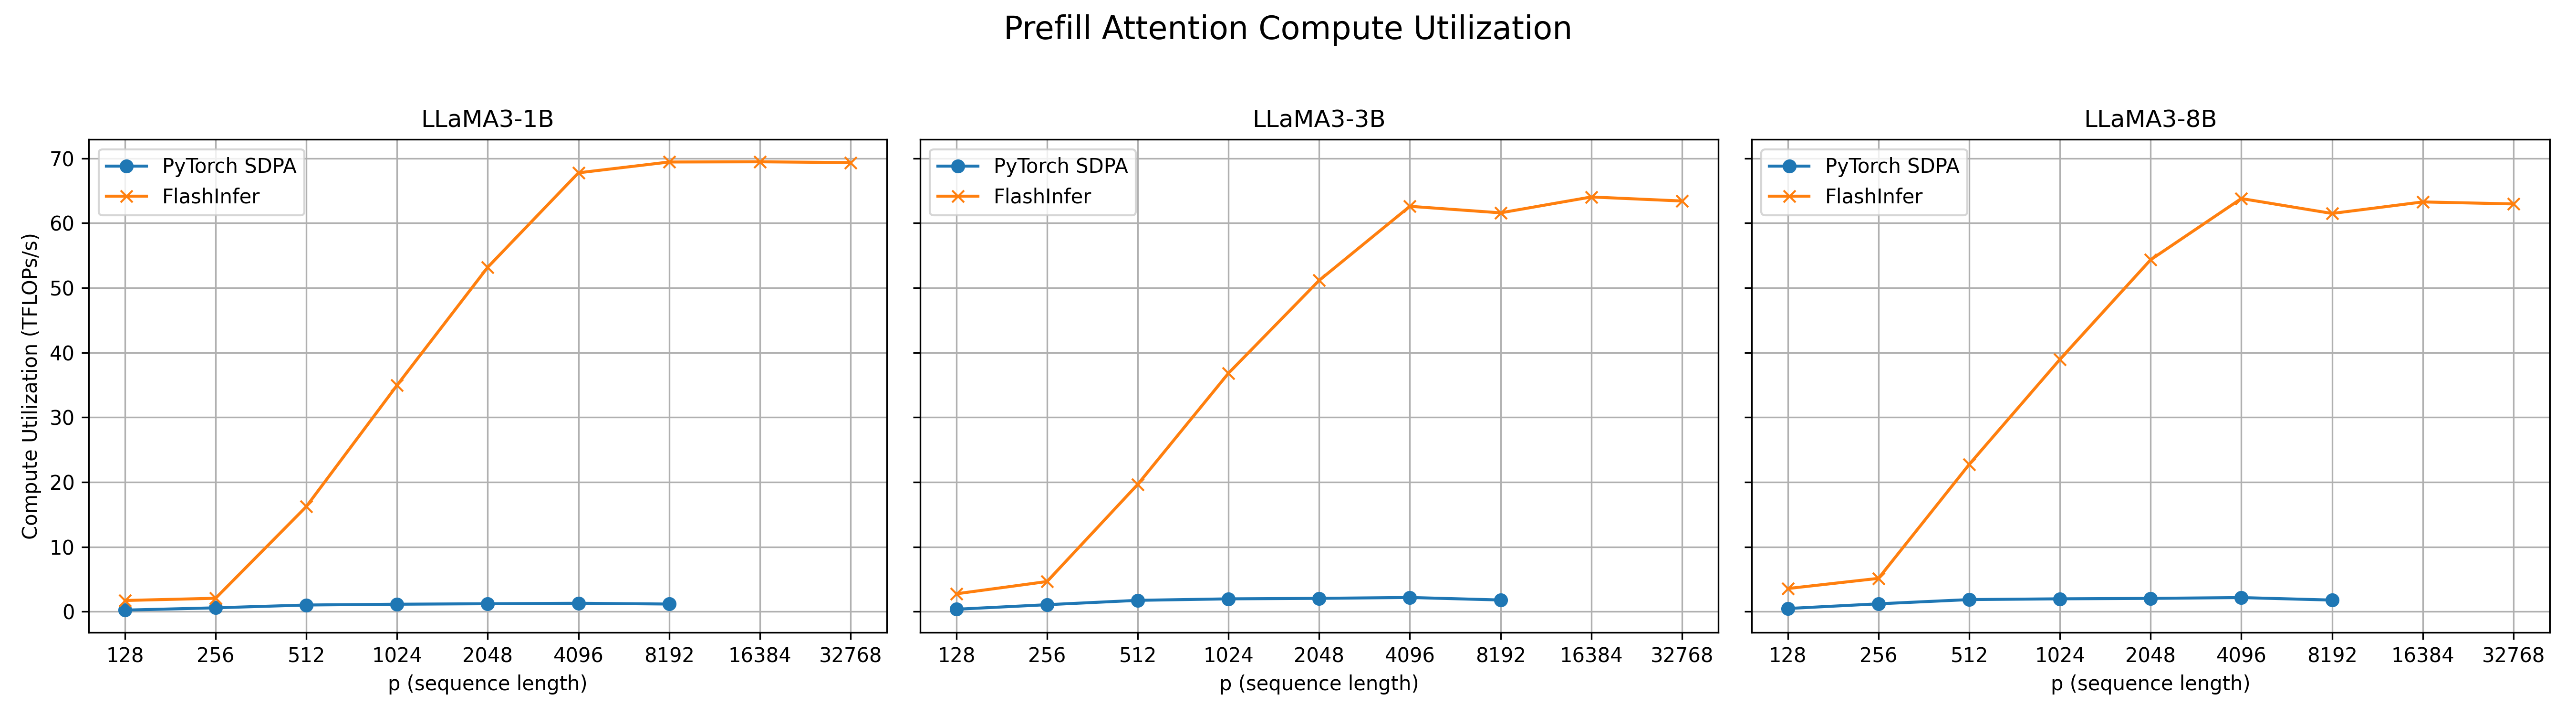
\includegraphics[width=\linewidth]{fig/prefill_attention_by_seq_len.png}
                \caption{%
                Compute utilization (TFLOP/s) for prefill attention for
                  LLaMA3-1B, LLaMA3-3B, LLaMA3-8B for a batch size of 1 and
                  sequence lengths between $2^{7}$ to $2^{15}$.
                }
                \label{fig:attention:prefill_seq}
            \end{figure}

            Our results are shown in Figure \ref{fig:attention:prefill_seq}. \\
            
            \item Batch size = $2^0 - 2^6, p = 1024$ for all three models.\\

            \begin{figure}[ht!]
                \centering
                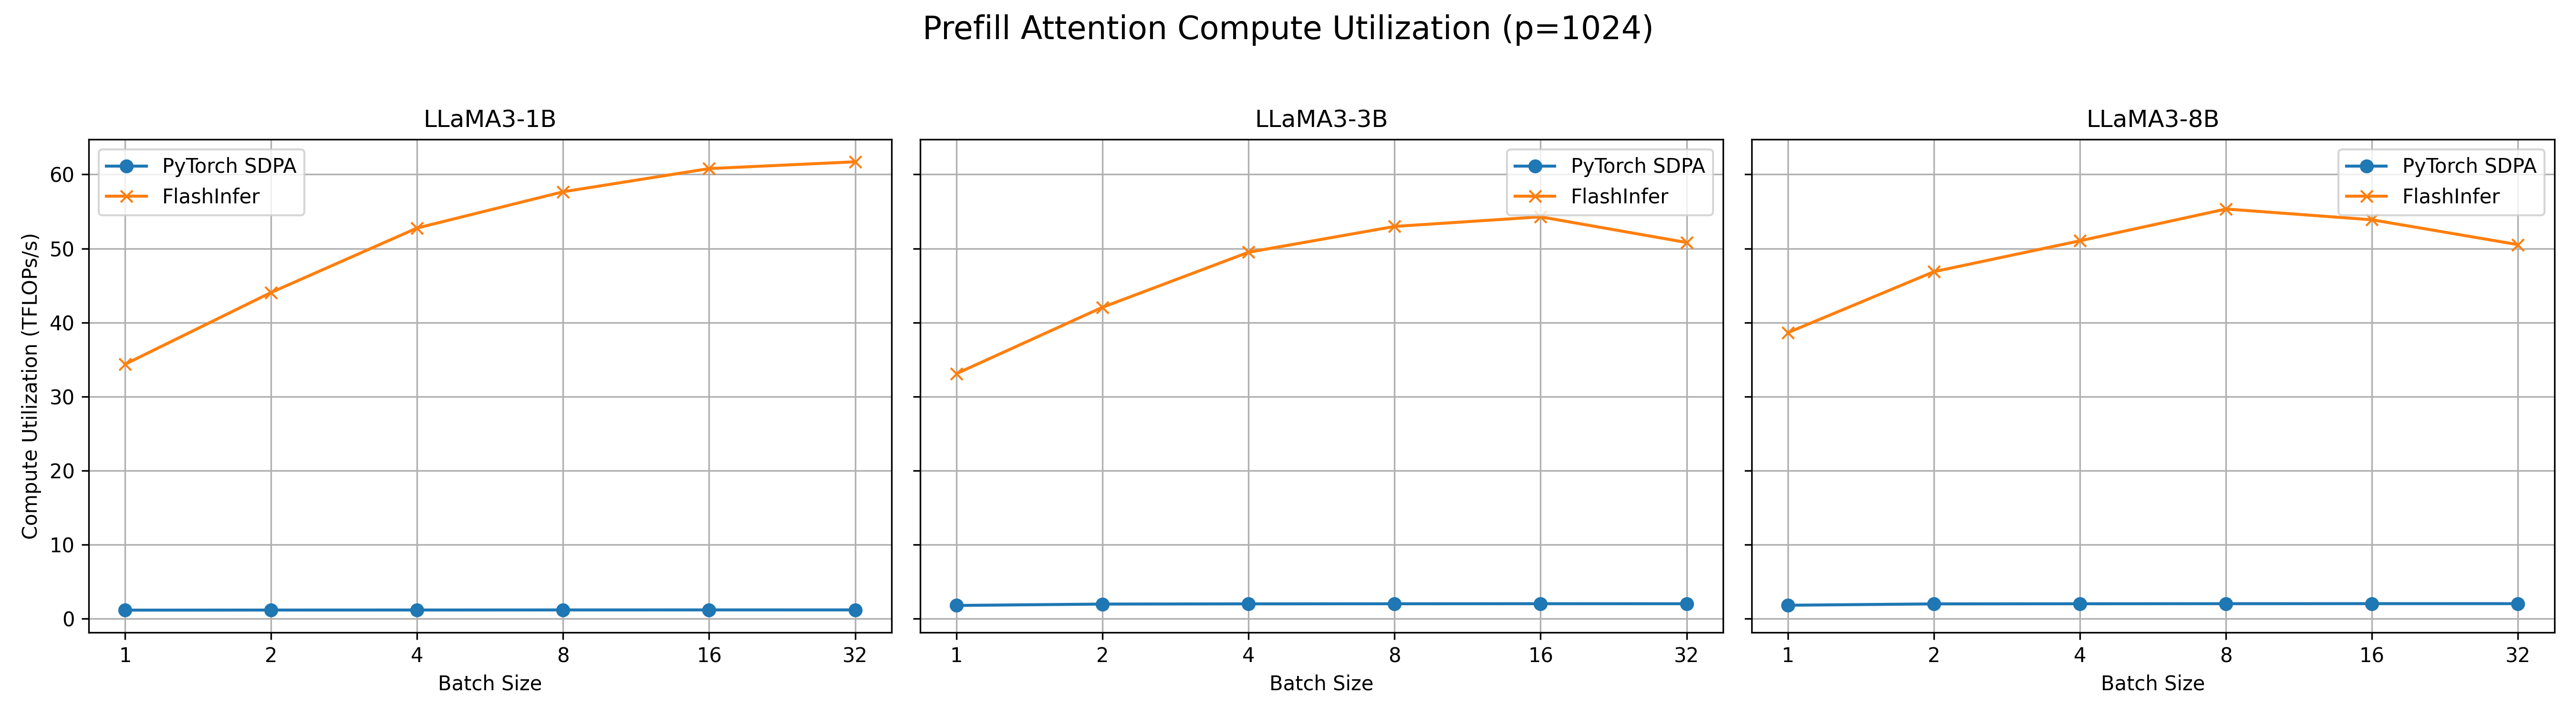
\includegraphics[width=\linewidth]{fig/prefill_attention_by_batch_size.png}
                \caption{%
                Compute utilization (TFLOP/s) for prefill attention for
                  LLaMA3-1B, LLaMA3-3B, LLaMA3-8B for a batch sizes from 1 to 32 and a sequence length of 1024.
                }
                \label{fig:attention:prefill_batch}
            \end{figure}

            Our results are shown in Figure \ref{fig:attention:prefill_batch}. \\

        \end{enumerate}

        \item Evaluate the decode attention performance of one layer
          using torch SDPA and FlashInfer.
          Plot memory bandwidth utilization (GB/s) similar to
          previous questions.

        \begin{enumerate}
            \item Batch size = 1, $c = 2^7 - 2^{15}$.\\

            Our results are shown in Figure \ref{fig:attention:decode_seq}.

            \begin{figure}[ht!]
                \centering
                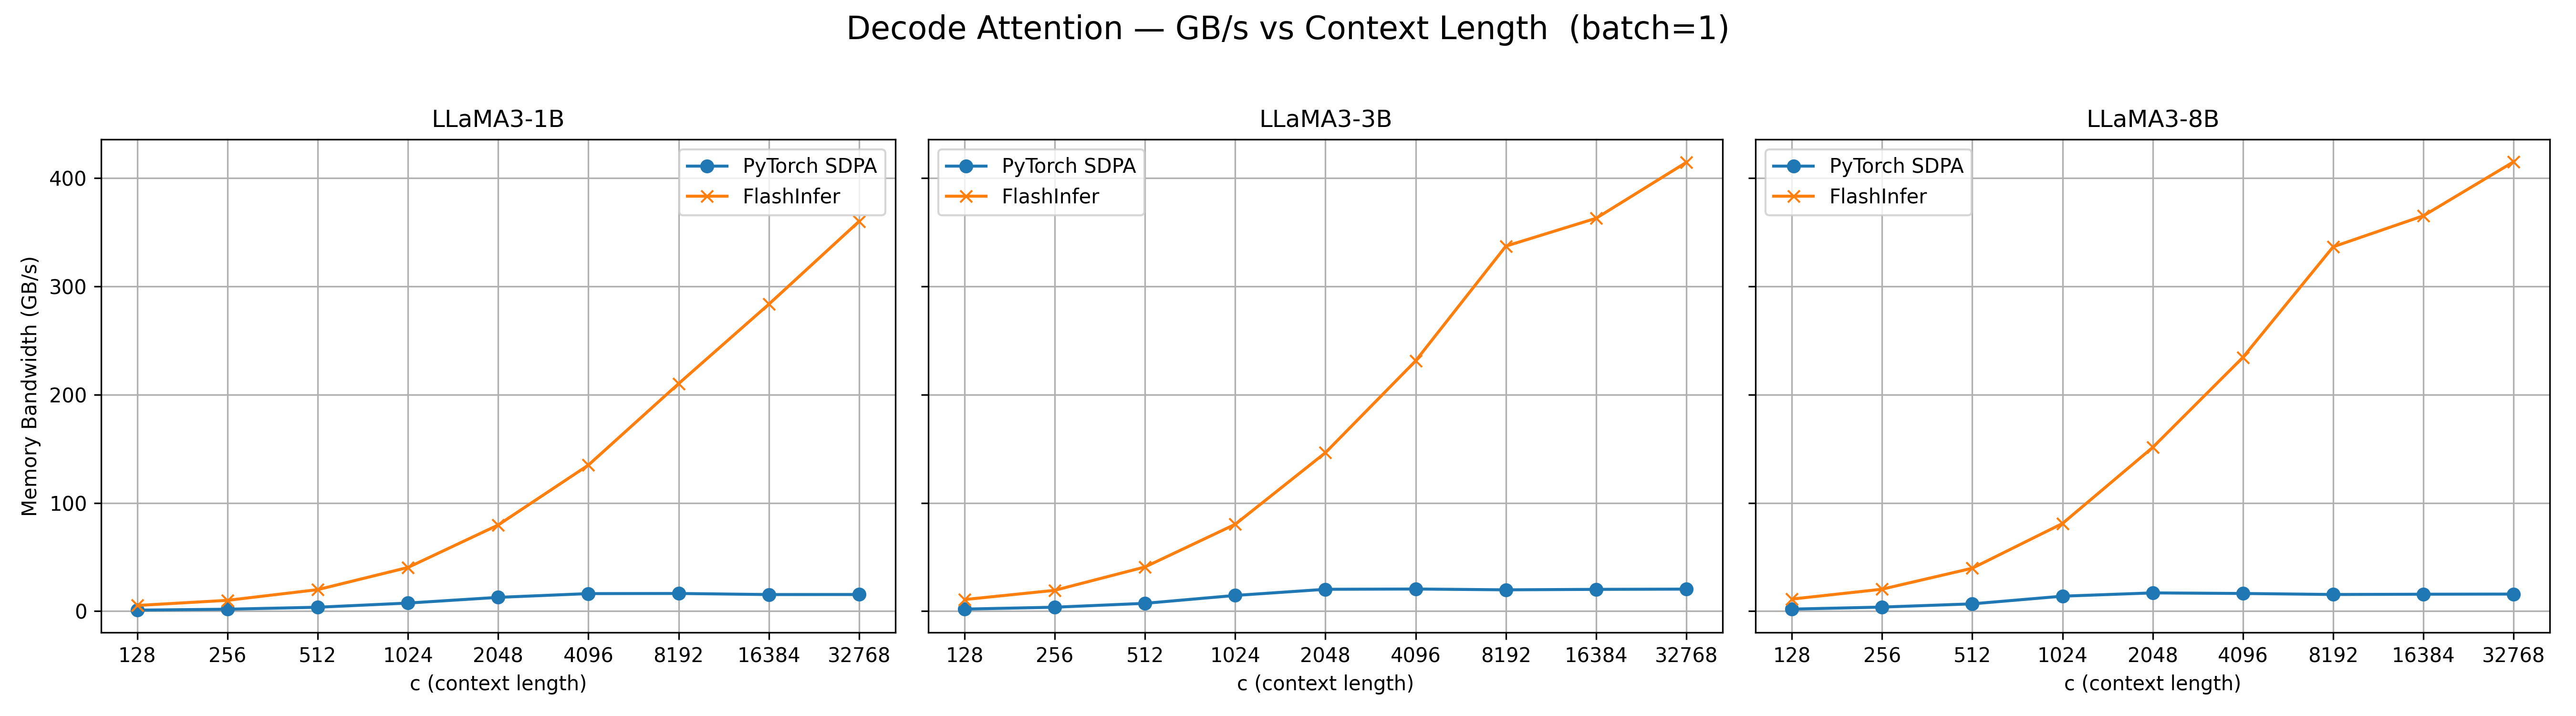
\includegraphics[width=\linewidth]{fig/decode_attention_by_context_len.png}
                \caption{%
                Memory bandwidth utilization (GB/s) for decode attention for
                  LLaMA3-1B, LLaMA3-3B, LLaMA3-8B for a batch size of 1 and
                  context lengths between $2^{7}$ to $2^{15}$.
                }
                \label{fig:attention:decode_seq}
            \end{figure}
            
            \item Batch size = $2^0 - 2^6, c = 1024$ for all three models. \\

            Our results are shown in Figure \ref{fig:attention:context_batch}. \\

            \begin{figure}[ht!]
                \centering
                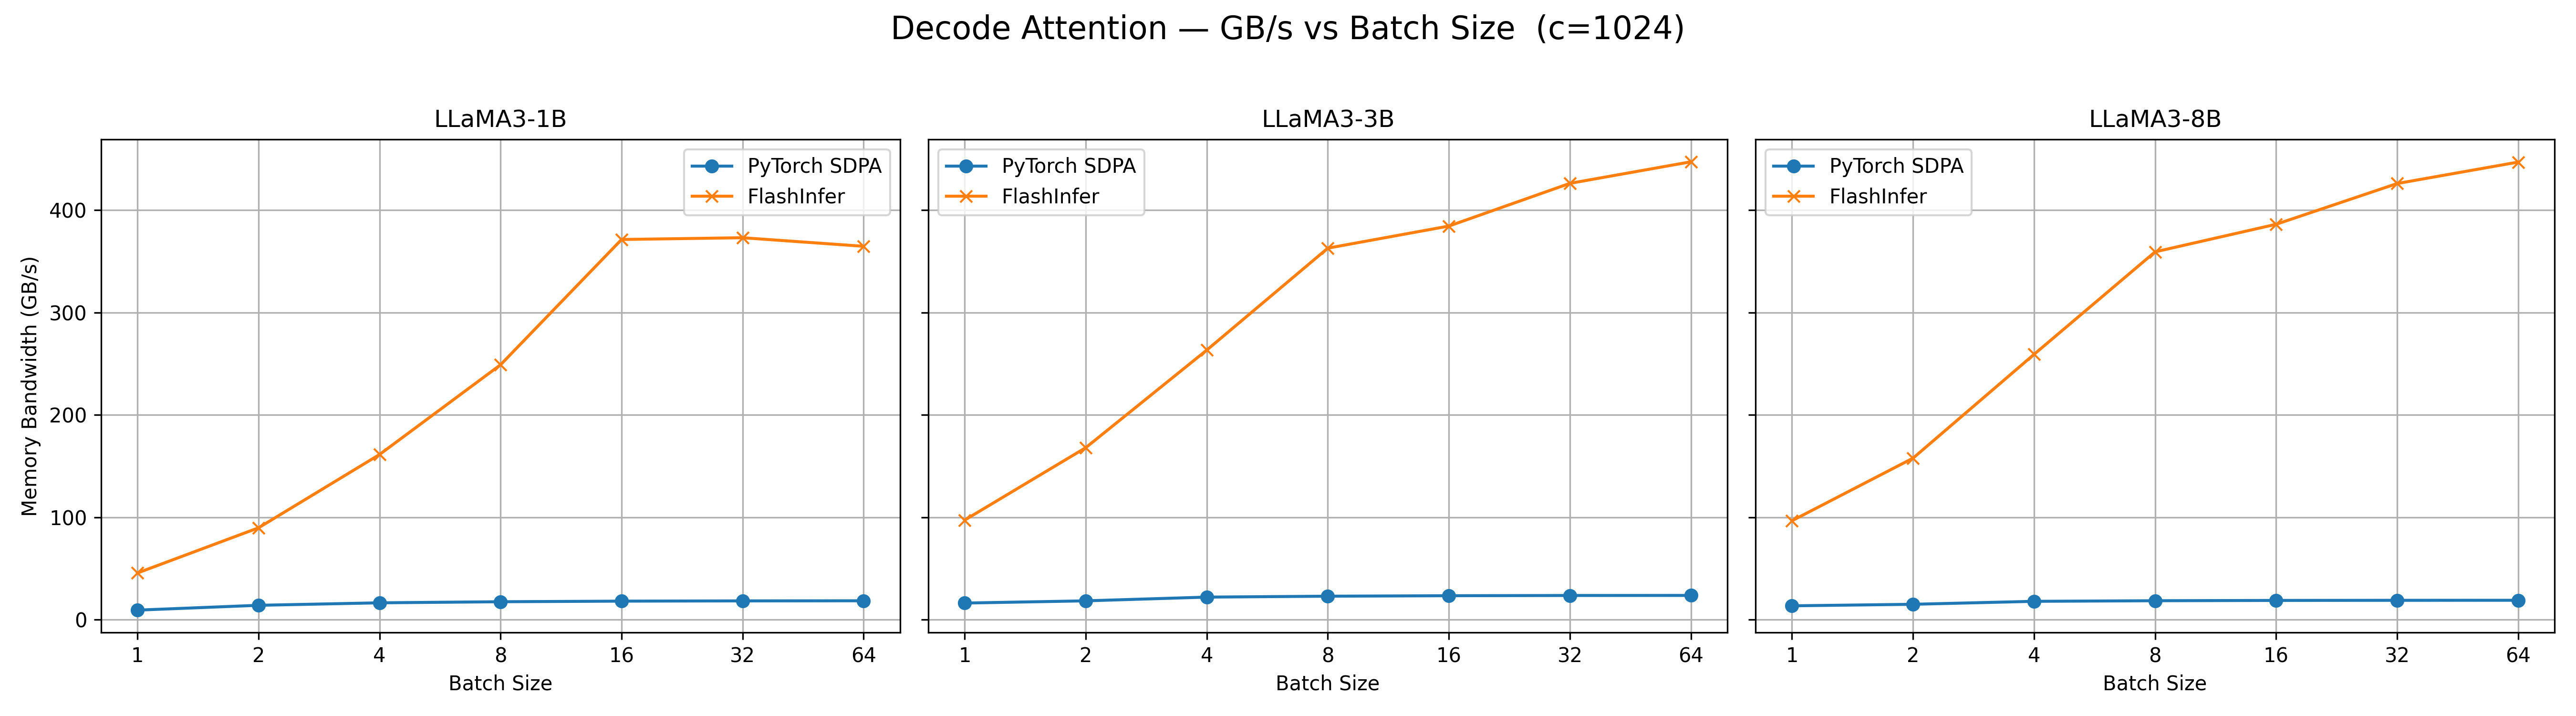
\includegraphics[width=\linewidth]{fig/decode_attention_by_batch_size.png}
                \caption{%
                Memory bandwidth utilization (GB/s) for decode attention for
                  LLaMA3-1B, LLaMA3-3B, LLaMA3-8B for a batch sizes from 1 to 32 and a context length of 1024.
                }
                \label{fig:attention:context_batch}
            \end{figure}
            
            \item Batch size = 128, c = 1024, page size = 1, 2, 4, 8, 16
            for all three models using FlashInfer.\\

            Our results are shown in Figure \ref{fig:attention:context_page}.

            \begin{figure}[ht!]
                \centering
                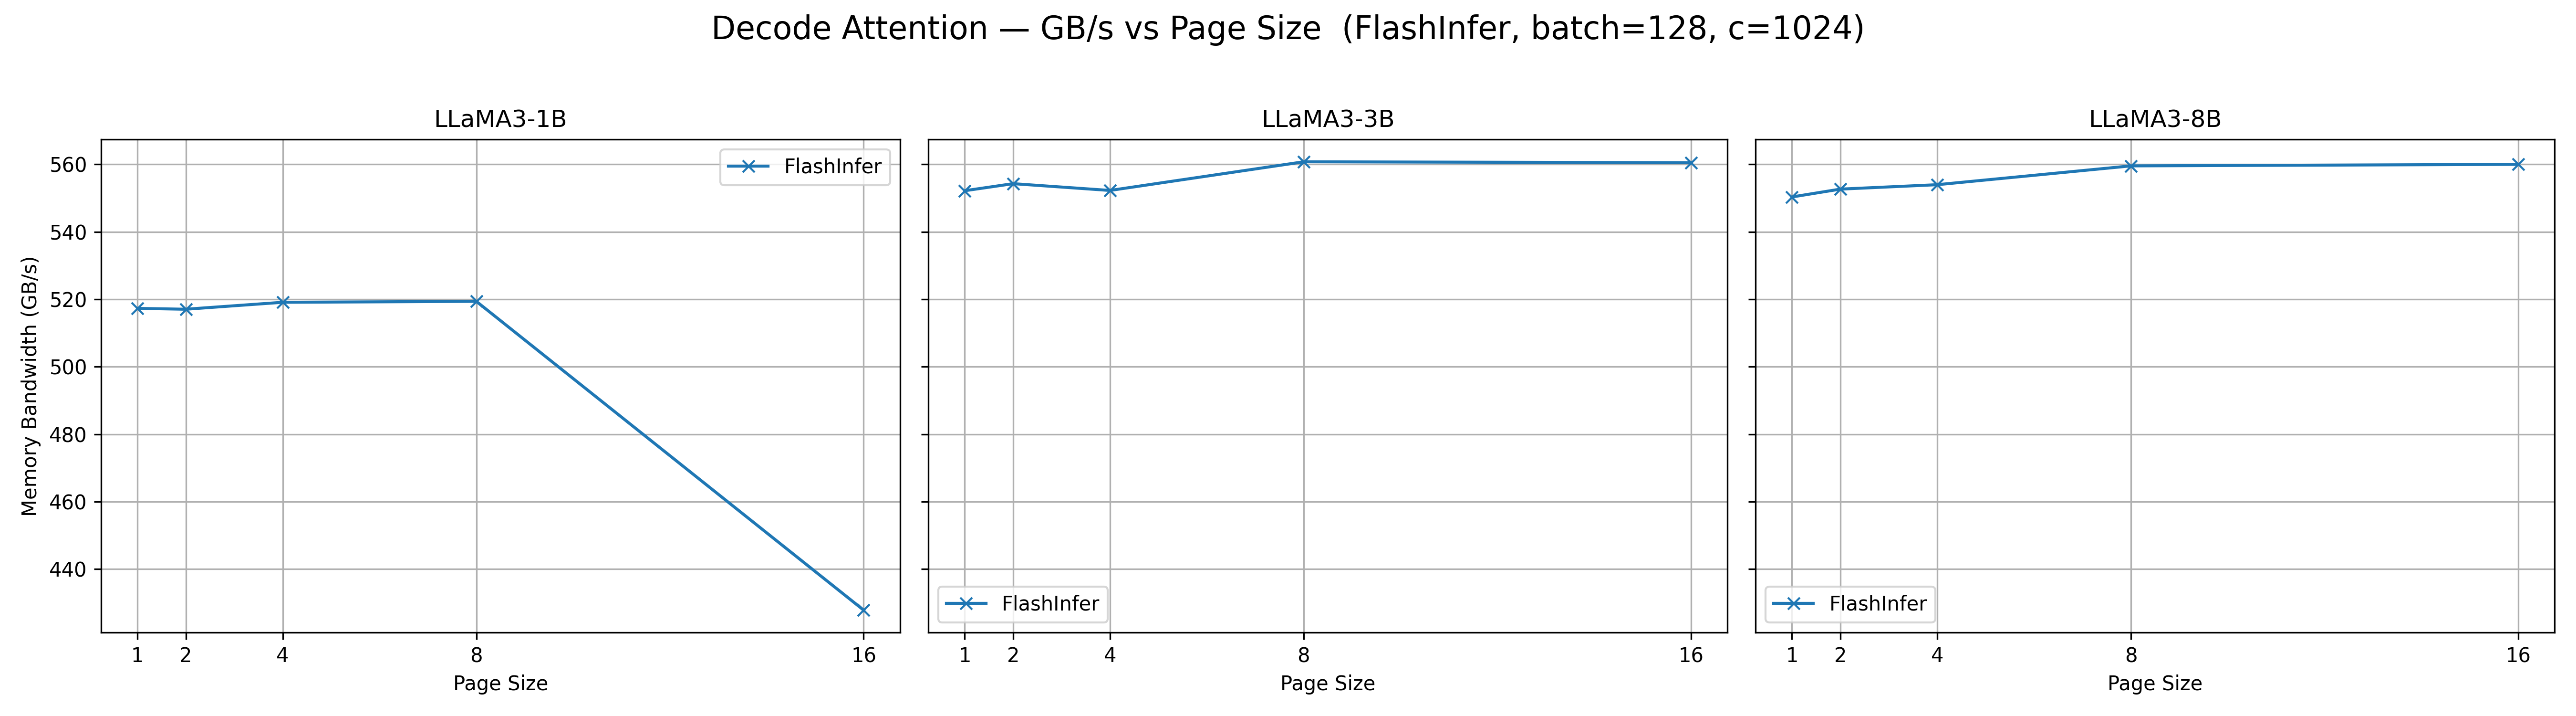
\includegraphics[width=\linewidth]{fig/decode_attention_by_page_size.png}
                \caption{%
                Memory bandwidth utilization (GB/s) for decode attention for
                  LLaMA3-1B, LLaMA3-3B, LLaMA3-8B for a batch size of 128,
                    a context length of 1024 and page sizes of
                    1, 2, 4, 8, and 16.
                }
                \label{fig:attention:context_page}
            \end{figure}
            
        \end{enumerate}
    \end{enumerate}
\end{enumerate}

% --- Section 3: End-to-end Performance ---
\section{End-to-end Performance}

\begin{enumerate}[label=\textbf{Q\arabic*.}]
    \item Starting from the \texttt{Section3/flashinfer\_pipeline.py}, construct a serving engine using FlashInfer attention and rope kernels with paged attention. \\

    \item 
    \begin{enumerate}
        \item With batch size 32, prefill length 256, decode length $2^5 - 2^{10}$, profile the prefill time and total decode time. Plot end-to-end time curve with the log(decode length) as the x-axis. Which phase is the key bottleneck? In the last decode cycle, which operation takes the longest time for different decode lengths? \\

        Our results are shown in Figure \ref{fig:e2e:decode}.
        Decode takes significantly longer than prefill. The largest bottleneck is the prefill attention kernel provided by FlashInfer, which used about $54\%$ of compute time. With low amounts of decode lengths, GEMM and the attention kernel aare about tied for the most longest operation (both around $33\%$ of time spent). However, as decode length increases, the attention kernel begins to take relatively much longer than GEMM.

        
        \begin{figure}[h!]
            \centering
            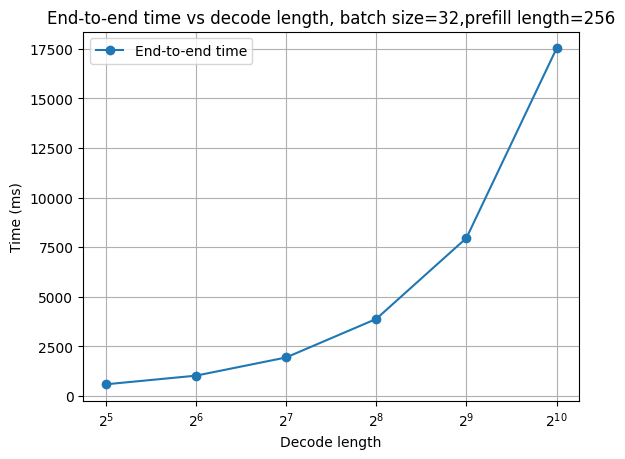
\includegraphics[width=0.8\linewidth]{fig/hw3_decode.png}
            \caption{End-to-End time vs. Decode Length.}
            \label{fig:e2e:decode}
        \end{figure}
                
        \item With batch size 1, prefill length $2^8 - 2^{14}$, profile the prefill time. Plot end-to-end time curve with log(prefill length) as x-axis. Examine the prefill time breakdown. What operations are the dominating factor for various prefill lengths? \\

        

        Our results are shown in Figure \ref{fig:e2e:prefill}. At batch sizes $2^8 - 2^{10}$, GEMM operations are the dominating factor. However, at batch sizes $2^{11}-2^{13}$, prefill attention kernels begin to take longer, and with batch size $2^{14}$, the prefill attention kernel is dominating operation in terms of end-to-end time.

        \begin{figure}[h!]
            \centering
            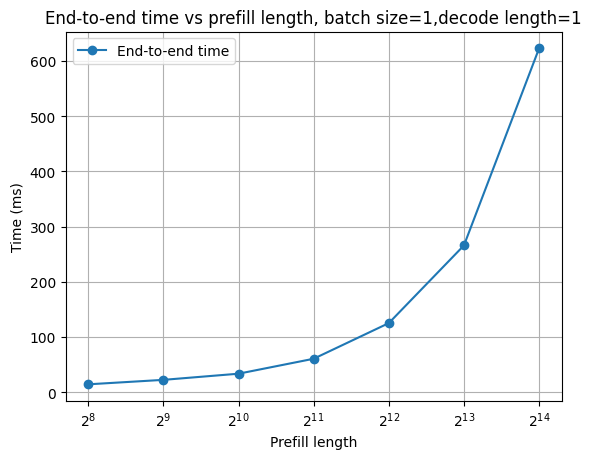
\includegraphics[width=0.8\linewidth]{fig/hw3_prefill.png} 
            \caption{End-to-End time vs prefill length.}
            \label{fig:e2e:prefill}
        \end{figure}

        \item With batch size $2^0 - 2^8$, prefill length 128, decode length 128, plot the end-to-end time curve with log(batch size) as x-axis. Plot the total throughput ((prefill + decode) / time) curve with log(batch size) as x-axis. When does the performance saturate? \\

        \begin{figure}[h!]
            \centering
            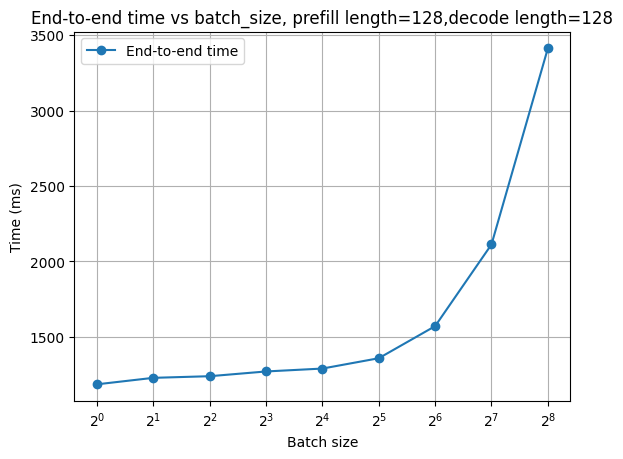
\includegraphics[width=0.45\linewidth]{fig/hw3_batch_size_time.png}
            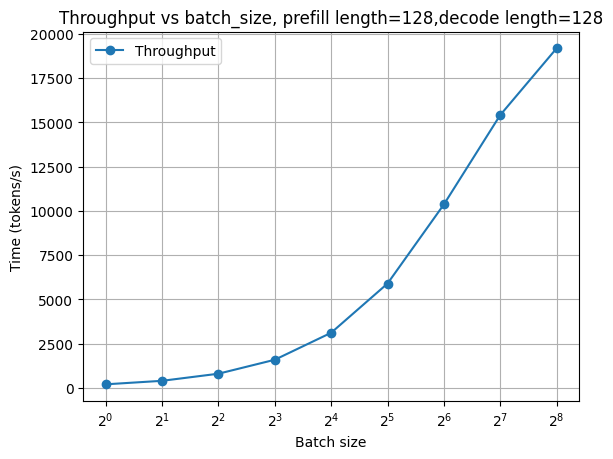
\includegraphics[width=0.45\linewidth]{fig/hw3_batch_size_throughput.png}
            \caption{Left: End-to-End runtime vs batch size. Right: token throughput vs batch size.}
            \label{fig:e2e:throughput}
        \end{figure}

         Our results are shown in Figure \ref{fig:e2e:throughput}.
        The model's performance begins to saturate at a batch size of $2^7$, where the throughput starts to decrease, and the time noticeably begins to increase between $2^7$ and $2^8$.
    \end{enumerate}
    
\end{enumerate}

\printbibliography

\end{document}